\subsection{Attitude Determination and Control System (ADCS)}

The purpose of the ADCS (Attitude Determination and Control System) is to control
the orientation of a satellite with respect to an inertial frame of reference or
another entity such as stars, planets, other celestial bodies and certain fields.
An attitude system comprises of several components including, sensors, actuators,
avionics, algorithms and software \cite{ADCS_nasa}. An ADCS can come in the form of both passive
and active systems depending on the nature of the mission and the subsequent
requirements of each operational mode. Within this section the design process used
for this spacecraft mission is explained.

\subsubsection{Design process}
A design process is essential to facilitate the effective and optimised selection
of the hardware and software required to create the ADCS subsystem. The design
process utilised for this project can be seen in figure \ref{fig:adcs_design}.
The iterative loop placed within the Figure is symbolic of the mindset that was
taken throughout this system’s design, with the understanding of the various
requirements and constraints changing throughout the process with information
feeding in from the design of other subsystems.

\begin{figure}[h]
	\centering
	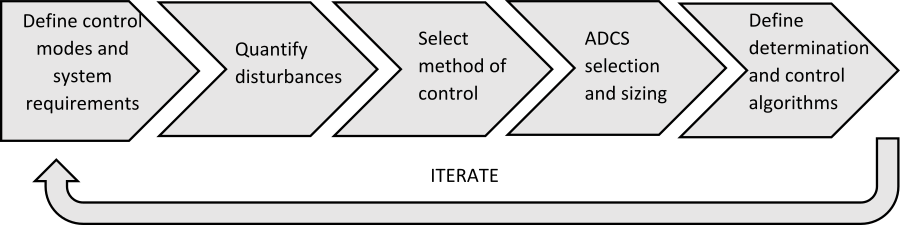
\includegraphics[width=\textwidth]{img/ADCS_design.png}
	\caption{Design process of the spacecraft ACDS}
	\label{fig:adcs_design}
\end{figure}

\subsubsection{Subsystem requirements}

When establishing the control modes and system requirements at the initial stage,
it was to consider what was needed to fulfill the mission objectives. Therefore,
some of the inputs into this design stage were the; mission requirements, mission
profile and mission constraints (cost, size and weight) etc. From this an initial
set of functional and performance requirements were set detailing the required
accuracy, reliability, rate of slew and others, useful in the later method of
control step.

\subsubsection{Control modes}

\paragraph{Detumble mode}

This mode is essential directly after the initial deployment of the satellite
constellation from the launch vehicle so stabilise the rotation of the satellites.
This mode also serves the purpose of a safe operating mode during the operational
life of the satellite, in the case of substantial disturbance torques, so that
the satellite’s rotation may be re-stabilised. It is preferable for de-tumbling
to occur as quickly as possible, so that the satellite can be returned to a useful state.

\paragraph{Operational mode}

Within this mode the satellite’s primary antenna must be directed over the earth’s
surface to enable data transmission and receipt with ground stations and devices.
This mode will also allow inter satellite communications between other satellites
due to the positioning of the secondary antenna’s. Within this stage the ADCS
requirements in terms of orientating the satellite are reduced, with only 2 axis
controls required to ensure the satellite antenna points directly to earth.

\paragraph{Thruster pointing mode}

This mode is needed during the early stages of the mission, post deployment,
whereby the satellites need to be positioned equidistant along their shared orbital
planes. It is preferable for thruster pointing to be as accurate as possible, so
as to minimise the required $\Delta V$ and thereby minimising the mission fuel requirement.
This mode may also be employed later in the life of the satellite, if fuel reserves remain.

\subsubsection{ADCS performance requirements}

With the control modes now defined to a basic extent in the previous paragraphs, performance requirements for each need to be considered to feed into the attitude control method selection such as; accuracy, range, jitter, drift and transient response \cite{ADCS_nasa}. These requirements can also incorporate input from other areas in the satellite such as sizing constraints from the structural side and powering constraints from the EPS. The formulation of these requirements is an iterative process, with the requirements themselves flexible to change as the mission profile is better understood and thereby the specific performance requirements that the CubeSat must fulfil are better established.

\subsubsection{Disturbances}

The disturbance environment in which the spacecraft will operate helps to determine which types of control methods will be required. For LEO spacecraft, such as the satellite being designed within this project, there are four key types of disturbance torques that need to be considered; gravity-gradient effects, magnetic field torques, solar radiation pressures and aerodynamic torques. The magnitudes of these disturbances depend on a variety of parameters including orbital altitude and plane inclination. Within this mission for example, the nature of the 8 different polar orbital planes employed for the constellation will mean that some of the CubeSats will receive more sun radiation compared to others which in turn means a variation in solar radiation pressure disturbances throughout the constellation.
The mass distribution and shape of the CubeSat are important in determining the centre of mass and the centre of pressure respectively. It’s ideal that for all orientations of the spacecraft relative to aerodynamic and sun radiation pressure disturbances, that the centre of pressure is as close to the centre of mass as possible to minimise the resultant disturbance moments. With the orbital height known (625 km), some early approximations and assumptions for these disturbances could be modelled and the values generated can be used in ADCS control method selection. Disturbances from gravity-gradient effects will be less prevalent throughout the life of these nanosatellites, due to their small size and symmetry pointed directly the earth, the adjusted centre of gravity will be in line with the satellites centre of mass.

In regard to internal disturbances; thruster misalignment during the orbital plane separation phase as well as reaction wheel friction and Electromotive force could create torque disturbances that would impact the attitude and stability of the spacecraft.

\subsubsection{Attitude Control Methods}

Based on the requirements created by the need for a thruster pointing mode, it
is clear that a solely passive system, of utilising the disturbance environment
itself to orientate the vehicle will not provide sufficient control or accuracy
with a typical +/- \SI{5}{\degree} and the 2 axis control possible from
gravity-gradient and passive magnetic techniques \cite{ADCS_nasa}.
A basic level active technique, spin stabilisation, offers a 2-axis solution that
may be sufficient for providing the pointing accuracy needed for the thruster
pointing mode. The symmetrical nature to the design of this CubeSat would allow
for full functionality within any of its operating modes with the spin even
potentially solving issues from induced internal disturbances due to thruster
misalignment. With an approximate accuracy of around +/- \SI{1}{\degree} it could
be more than suitable for thruster pointing however, due to the gyroscopic stiffness
resulting from the spinning motion, re-pointing could be very slow \cite{ADCS_nasa}.
Further study may be required to evaluate whether a requirement for minimum slew rates exists.
An alternative solution if slew rate requirements are too high could be a zero-momentum
system such as a combination of reaction wheels and magnetic torquers.
The reaction wheels could provide a similar accuracy to that of the spin
stabilization method, with the magnet torquers required as a method of desaturation
of the stored angular momentums. A worry with this system may be the sizing within
a 3U CubeSat, however an example of a system with 3 orthogonal reaction wheels and
two magnetorquers was found with only 10\% of the total 3U structure volume taken
up \cite{Delfi-n3xt}.

\subsubsection{Selection and Sizing of ADCS Hardware}

With some potential options of ADCS control methods mentioned in the previous section,
what needs to come next is the specific selection and sizing of both actuator and
sensor hardware. In selecting actuator hardware there are a variety of factors that
need to be considered, firstly the torque requirements but also in the case of
moving parts such as reaction wheels, the characteristics of vibrations that could
lead to Jitter.

With actuation methods considered, it is also very important for attitude
determination methods to be carefully selected. Sun sensors, with their high
accuracy and relatively low power requirement provide a good starting point
for the attitude determination element of the system. With a combination of
5-6 sensors allowing for optimised performance and sufficient redundancy.
\cite{Delfi-n3xt} The clear disadvantage with these sensors is however that
with the planned orbit of the CubeSat’s within this mission, they will all spend
a period of time where a view of the sun is not available. To provide determination
data during eclipse conditions, magnetometers could be utilised with their low power
usage and with the proposed low earth orbit however they can lack accuracy, typically;
+/- \SI{0.5}{\degree} to +/- \SI{3}{\degree}. If during future analysis a greater attitude
determination accuracy becomes a requirement, horizon sensors could be employed
with accuracy’s between +/- \SI{0.01}{\degree} and +/- \SI{0.1}{\degree} for a
fixed head sensor configuration. They can however bring with them a greater power
requirement from the EPS.

\subsubsection{Define Determination and Control Algorithms}

Finally, after putting some consideration into the previous parts of the design process, it’s also important that the algorithms that bring the hardware together is studied. Whilst this has not been covered yet within the scope of this report this would form the ‘further work’ element, essential so that an initial prototype of the full ADCS system could be modelled using mathematical simulations but also the tools of linear servomechanism theory. Modelling would take place starting at a basic level, focusing on constructing a control system for only 1 axis of motion, before progressing it into the inclusion of full 2 axis of 3 axis control.
